\documentclass{article}
\usepackage{graphicx, float}
\usepackage{enumitem}
\usepackage[hidelinks]{hyperref}

\graphicspath{{images/}}
\author{Cristian Di Cintio - S1110150 \and Federico Di Giovannangelo - S0000000}
\date{}

\title{READING STATS\par \large RELAZIONE DI PROGRAMMAZIONE MOBILE}


\begin{document}

\maketitle
\tableofcontents
\newpage

\section{Introduzione}

L'applicazione sviluppata ha come obiettivo la memorizzazione delle statistiche di libri in lettura dell'utente. Tali statistiche riguardano la percentuale di completamento del libro e il tempo impiegato, memorizzato per ciascuno libro.

L'utente per usufruire delle funzionalità dell'app deve registrarsi con nome, cognome, email, username e password. Per lo username e l'email vengono effettuati dei controlli per verificare l'univocità e non permettere la registrazione di utenti con medesimo username o email.

In seguito l'utente può effettuare l'accesso con la propria email e password.

L'utente può ricercare i libri in un catalogo tramite la digitazione del titolo in una barra di ricerca o scansionando, con un pulsante apposito, il codice a barre di un libro fisico. In seguito può decidere di aggiungerlo in tre liste distinte, "da leggere", "in lettura" e "letti", 
per avere un resoconto delle pagine lette e del tempo impiegato nella lettura dei libri salvati. Il catalogo permette anche il filtraggio di libri tramite la selezione di categorie predefinite.

Al momento della lettura l'utente può avviare un timer per un libro in lettura, presente nell'omonima lista, e disattivarlo al termine della sessione.

L'utente può visualizzare e modificare i propri dati personali e interagire con altri utenti, visualizzando principalmente quali libri hanno salvato e quali stanno leggendo, ognuno con le loro rispettive metriche.

L'intera applicazione è stata sviluppata inizialmente in Kotlin per ambiente Android e in seguito in Flutter per un funzionamento multipiattaforma, in modo tale da permettere una maggiore compatibilità e una migliore interazione tra utenti con diversi dispositivi mobile.

Lo sviluppo in Kotlin è stato applicato con Jetpack Compose, per permettere uno sviluppo moderno e in linea con le attuali applicazioni sul mercato, con una struttura architetturale basata sul Model-View-ViewModel (MVVM) garantendo una composizione comprensibile per lo sviluppo dell'app.
Le informazioni principali dei libri vengono visualizzate tramite l'utilizzo di API fornite da Google Books.

\section{Progettazione e sviluppo Android}

\subsection{Requisiti}
Si riportano di seguito i requisiti \textit{funzionali} e \textit{non funzionali}
\subsubsection{Requisiti funzionali}

\begin{figure}[H]
  \centering
  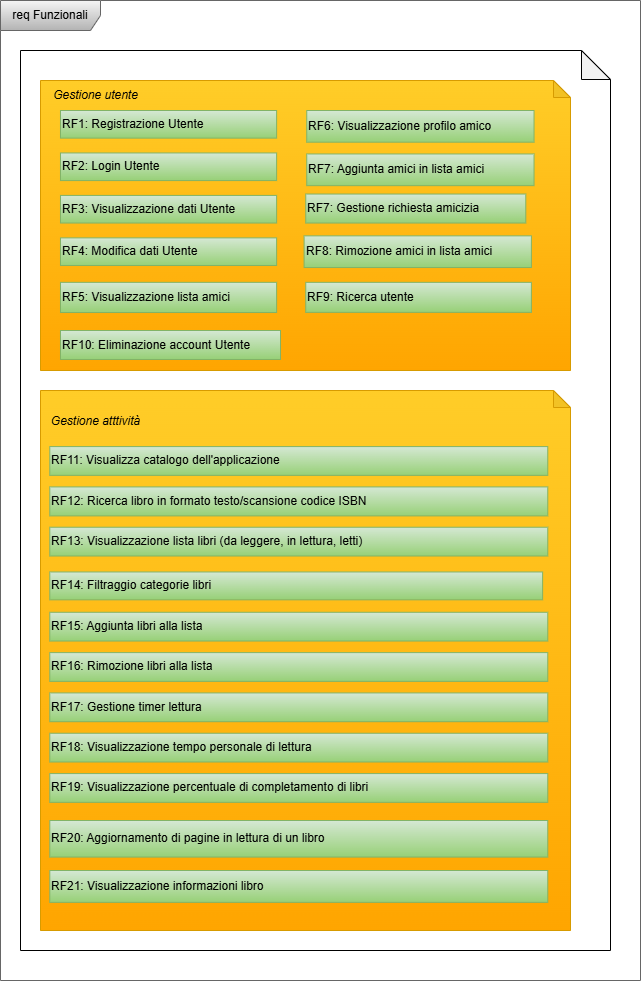
\includegraphics[width=.9\linewidth]{req_funzionali.png}
  \caption{Requisiti funzionali}
  \label{fig:sitemap}
\end{figure}

\begin{itemize}
    \item \textit{Gestione utente}
    \begin{itemize}
        \item \textit{RF1: Registrazione utente} - L'applicazione permette di registarsi con le proprie informazioni personali
        \item \textit{RF2: Login utente} - L'applicazione permette di autenticare l'utente registrato con le proprie informazioni personali
        \item \textit{RF3: Visualizzazione dati utente} - L'applicazione permette di visualizzare i propri dati personali
        \item \textit{RF4: Modifica dati utente} - L'applicazione permette di modificare i propri dati personali
        \item \textit{RF5: Visualizzazione lista amici} - L'applicazione permette di visualizzare la lista degli amici che hanno accettato la sua richiesta d'amicizia
        \item \textit{RF6: Visualizzazione profilo amico} - L'applicazione permette di visualizzare il profilo di un suo amico nella lista
        \item \textit{RF7: Aggiunta amici in lista amici} - L'applicazione permette di aggiungere un amico nella sua lista inviando una richiesta
        \item \textit{RF8: Gestione richiesta di amicizia} - L'utente può decidere se accettare o rifiutare una richesta di amicizia
        \item \textit{RF9: Rimozione amici da lista amici} - L'applicazione permette di rimuovere un amico dalla lista amici
        \item \textit{RF10: Ricerca utente} - L'applicazione permette di ricercare un utente digitando il suo username o nome completo
        \item \textit{RF11: Eliminazione account utente} - L'applicazione permette all'utente di cancellare il proprio profilo
    \end{itemize}
    \item \textit{Gestione attività}
    \begin{itemize}
        \item \textit{RF12: Visualizza catalogo dell'applicazione} - L'applicazione permette di visualizzare il catalogo dei libri distinti in categorie
        \item \textit{RF13: Ricerca libro in formato testo o tramite scansione codice a barre} - L'applicazione permette la ricerca del libro digitando testualmente il titolo in una casella di ricerca apposita oppure scansionando il codice a barre di un libro fisico
        \item \textit{RF14: Visualizzazione lista libri (da leggere, in lettura, letti)} - L'applicazione permette di visualizzare il contenuto delle liste principali formate dai libri salvati dall'utente
        \item \textit{RF15: Filtraggio categorie libri} - L'applicazione permette all'utente di filtrare le categorie dei libri da visualizzare nel catalogo 
        \item \textit{RF16: Aggiunta libri alla lista} - L'applicazione permette all'utente di aggiungere i libri in una delle apposite liste fornite dall'app
        \item \textit{RF17: Rimozione libri dalla lista} - L'applicazione permette la rimozione di libri dalle liste
        \item \textit{RF18: Gestione timer lettura} - L'applicazione permette di tenere sotto controllo il tempo di lettura di un libro con l'utilizzo di un timer dedicato attivabile e disattivabile dall'utente
        \item \textit{RF19: Visualizzazione tempo personale di lettura} - L'applicazione permette all'utente di visualizzare per ogni singolo libro il tempo di lettura impiegato con l'utilizzo del timer
        \item \textit{RF20: Visualizzazione percentuale completamento di libri} - L'applicazione permette di visualizzare la percentuale di completamento di ogni singolo libro, calcolata tramite il numero di pagine lette dall'utente rispetto al numero di pagine totali di un determinato libro
        \item \textit{RF21: Aggiornamento percentuale di pagine in lettura di un libro} - L'applicazione permette di aggiornare il numero di pagine lette di un libro per calcolare la percentuale di completamento
        \item \textit{RF22: Visualizzazione informazioni libro} - L'applicazione permette la visualizzazione delle info di un determinato libro 
    \end{itemize}
\end{itemize}

\subsubsection{Requisiti non funzionali}

\begin{figure}[H]
  \centering
  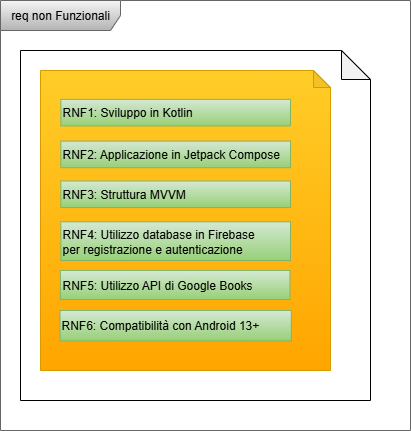
\includegraphics[width=.6\linewidth]{req_non_funzionali.png}
  \caption{Requisiti non funzionali}
  \label{fig:sitemap}
\end{figure}

\begin{itemize}[label=\textendash]
    \item \textit{RNF1: Sviluppo in Kotlin} - L'applicazione è stata sviluppata principalmente con il linguaggio di programmazione Kotlin
    \item \textit{RNF2: Applicazione in Jetpack Compose} - L'applicazione è stata realizzata con Jetpack Compose per realizzare le interfacce grafiche
    \item \textit{RNF3: Struttura MVVM} - L'applicazione ha una struttura architetturale basata su Model-View-ViewModel per agevolare la programmazione con sezioni dedicate
    \item \textit{RNF4: Firebase Firestore per memorizzazione e accesso/autenticazione utente} - L'applicazione fa utilizzo per la memorizzazione di dati e la gestione della registrazione e l'accesso dell'utente di un database tramite la piattaforma Google Firebase
    \item \textit{RNF5: API di Google Books} - L'applicazione si sincronizza e fa utilizzo delle API Key di Google Books per mostrare i libri nel catalogo e nella ricerca
    \item \textit{RNF6: compatibilità con Android 13+} - L'applicazione ha una compatibilità con il livello di API 33, permettendone l'utilizzo su android 13 e oltre
\end{itemize}

\subsubsection{Casi d'uso}
Si riportano gli attori e i tre casi d'uso principali che descrivono le azioni principali che si possono svolgere nell'applicazione a partire dai requisiti elencati in precedenza.

\begin{figure}[H]
  \centering
  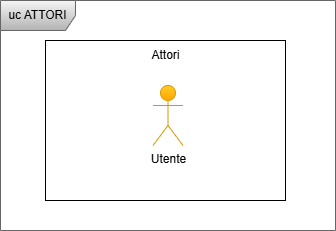
\includegraphics[width=.6\linewidth]{cu_attori.png}
  \caption{Attori principali}
  \label{fig:sitemap}
\end{figure}

\begin{figure}[H]
  \centering
  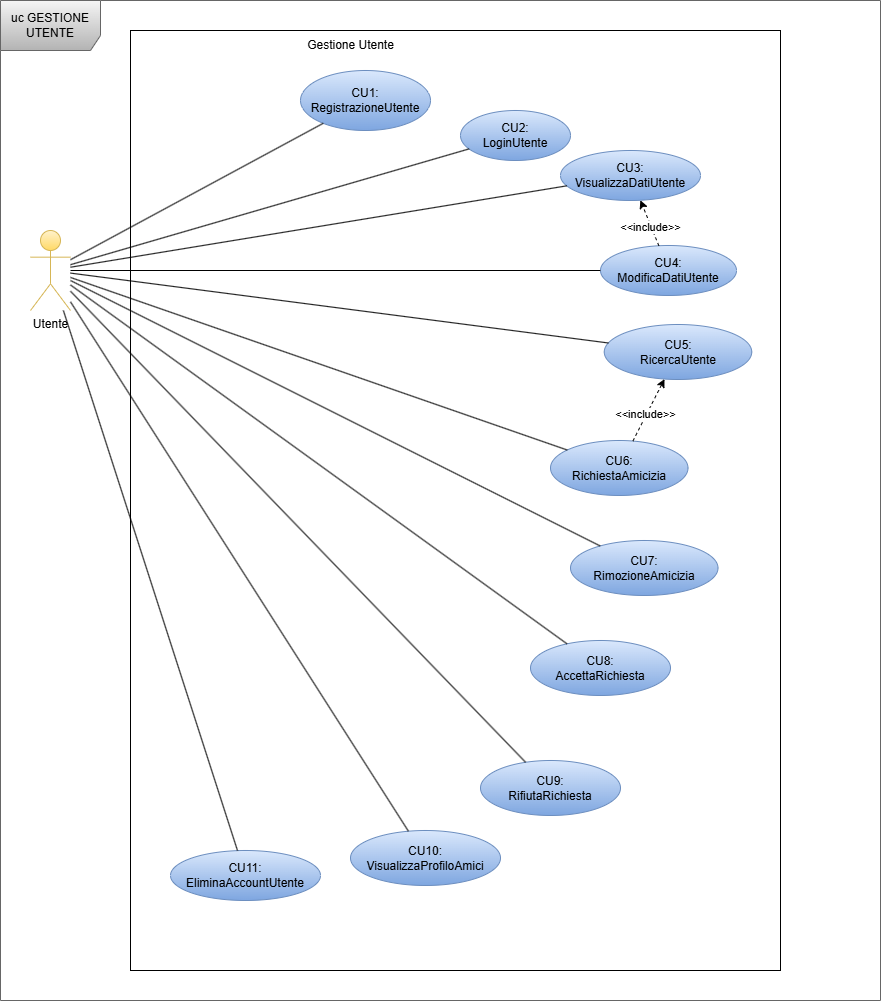
\includegraphics[width=.8\linewidth]{cu_utente.png}
  \caption{Gestione utente}
  \label{fig:sitemap}
\end{figure}

\begin{itemize}[label=\textendash]
    \item \textit{CU1: RegistrazioneUtente} - L'utente, per usufruire dei servizi offerti dall'applicazione, ha bissogno di registarsi con le proprie informazioni personali
    \item \textit{CU2: LoginUtente} - L'utente può accedere ai servizi forniti inserendo le proprie credenziali (email e password) precedentemente utilizzate per registrarsi
    \item \textit{CU3: VisualizzaDatiUtente} - L'utente può visualizzare le proprie informazioni personali in una sezione dedicata
    \item \textit{CU4: ModificaDatiUtente} - L'utente può modificare i propri dati personali
    \item \textit{CU5: RicercaUtente} - L'utente può ricercare un utente digitando il suo nome utente (usernam) o nome completo (nome e/o cognome)
    \item \textit{CU6: RichiestaAmicizia} - L'utente può aggiungere amici nella propria lista inviando richieste ad altri utenti
    \item \textit{CU7: RimozioneAmicizia} - L'utente può rimuovere gli amici dalla propria lista
    \item \textit{CU8: AccettaRichiesta} - L'utente può accettare la richiesta di amicizia da un altro utente che l'ha inviata
    \item \textit{CU9: RifiutaRichiesta} - L'utente può rifiutare la richiesta di amicizia da un altro utente che l'ha inviata
    \item \textit{CU10: VisualizzaProfiloAmici} - L'utente può visualizzare il profilo dei propri amici con le loro statistiche di lettura
    \item \textit{CU11: EliminaAccountUtente} - L'utente può eliminare il proprio account utente
\end{itemize}

\begin{figure}[H]
  \centering
  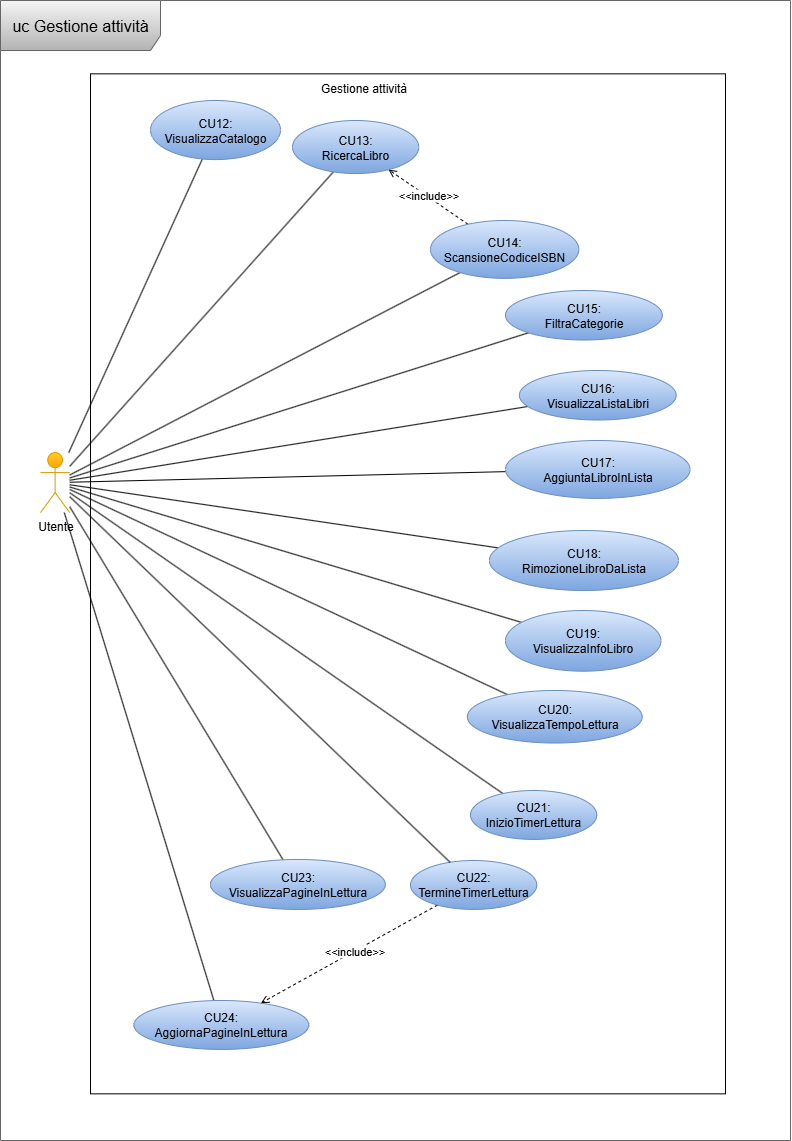
\includegraphics[width=0.72\linewidth]{cu_attivita.png}
  \caption{Gestione attività}
  \label{fig:sitemap}
\end{figure}

\begin{itemize}[label=\textendash]
    \item \textit{CU12: VisualizzaCatalogo} - L'utente può visualizzare il catalogo di libri separato in categorie
    \item \textit{CU13: RicercaLibro} - L'utente può ricercare il libro digitando il titolo nella barra di ricerca presente nel catalogo
    \item \textit{CU14: ScansioneCodiceISBN} - L'utente può effettuare la scansione del codice ISBN di un libro fisico tramite la fotocamera del telefono
    \item \textit{CU15: FiltroCategorie} - L'utente può filtrare le categorie del catalogo selezionandole da un lista con checkbox
    \item \textit{CU16: VisualizzaListaLibri} - L'utente può visualizzare una delle tre liste principali (da leggere, in lettura, letti) per memorizzare i libri salvati
    \item \textit{CU17: AggiuntaLibroInLista} - L'utente può aggiungere un libro selezionato in una delle tre liste principali (da leggere, in lettura, letti)
    \item \textit{CU18: RimozioneLibroDaLista} - L'utente può rimuovere un libro presente in una delle tre liste principali (da leggere, in lettura, letti)
    \item \textit{CU19: VisualizzaInfoLibro} - L'utente può visualizzare le informazioni principali che rappresentano il libro selezionandolo dal catalogo o dalle liste
    \item \textit{CU20: VisualizzaTempoLettura} - L'utente può visualizzare il tempo di lettura di un proprio libro
    \item \textit{CU21: InizioTimerLettura} - L'utente può iniziare la sessione di lettura di un libro tramite l'inizio di un timer dedicato
    \item \textit{CU22: TermineTimerLettura} - L'utente può terminare la sessione di lettura di un libro permettendo di fermare il timer
    \item \textit{CU23: VisualizzaPagineInLettura} - L'utente può visualizzare le pagine in lettura di un libro salvato nell'omonima lista
    \item \textit{CU24: AggiornaPagineInLettura} - L'utente può aggiornare le pagine 
\end{itemize}

\subsection{Architettura applicazione}

\subsubsection{MVVM}

Per la struttura dell'applicazione è stato scelto il pattern architetturale Model-View-ViewModel (MVVM) per ottenere
una separazione netta delle responsabilità tale da rendere il codice scalabile e facilmente aggiornabile.
Le sue principali componenti sono:
\begin{itemize}
  \item \textbf{Model:} Gestisce i dati dell'applicazione e della loro persistenza, principalmente in remoto con Firebase nel caso specifico di questa applicazione, 
  permettendo operazioni di accesso, modifica e salvataggio dei dati per gli \textit{utenti} che si registrano e dei \textit{libri} che salvano in determinate liste. 
  \item \textbf{View:} Rappresenta le interfacce dell'applicazione per permettere all'utente di interagire con la logica dell'applicazione. 
  Vengono definite tramite funzioni con la notazione iniziale \textit{@Composable} e possono essere richiamate nel file contenente il MainActivity o in altre funzioni con la stessa notazione.
  \item \textbf{ViewModel:} Funge da intermediario tra View e Model e permette il cambiamento dello stato della UI con le interazioni dell'utente tramite \textit{LiveData}
\end{itemize}

\subsubsection{Diagramma delle componenti}

Il seguente diagramma di componenti rappresenta le principali istanze e le loro interazioni, in particolare tra l'utente e un singolo libro scelto, la lista dei libri e la richiesta di amicizia verso un altro utente.
Per il libro l'utente può decidere se inserirlo in una lista o rimuoverlo, mentre per la richiesta l'utente può inviarne una e visualizzarne una ricevuta, per poi decidere se accettarla o rifiutarla.

\begin{figure}[H]
  \centering
  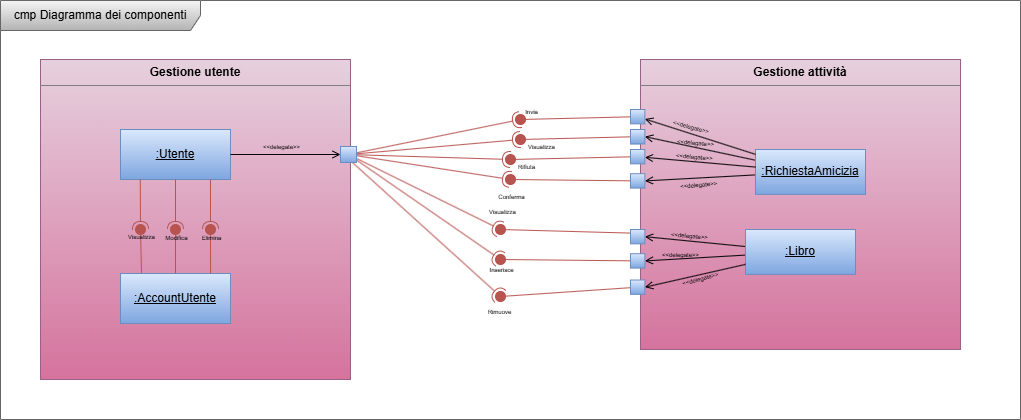
\includegraphics[width=1\linewidth]{diagramma_componenti.png}
  \caption{Diagramma delle componenti}
  \label{fig:sitemap}
\end{figure}

\subsection{Gestione Database - Firebase}
In presenza di un sistema di autenticazione e registrazione a un servizio online, con la possibilità per l'utente di interagire con altri utenti, e permettere il salvataggio personale di libri nel proprio profilo,
l'infrastruttura migliore per manipolare questi dati risulta essere il database gestionale Firestore di Google Firebase.

Firestore è un DB NoSQL strutturato a documenti, il quale permette il salvataggio di dati in documenti raggrupati in collezioni e può contenere sottocollezioni e campi annidati. Tali documenti e collezioni vengono generati con la scrittura di dati tramite codice.

Il suo utilizzo si concentra su due componenti della sezione \textit{Creazione}:
\begin{itemize}
  \item \textit{Authentication:} permette di gestire il metodo di accesso degli utenti tramite diversi servizi. Nel caso di questo progetto abbiamo implementato esclusivamente l'autenticazione semplice tramite email e password.
    \begin{figure}[H]
    \centering
    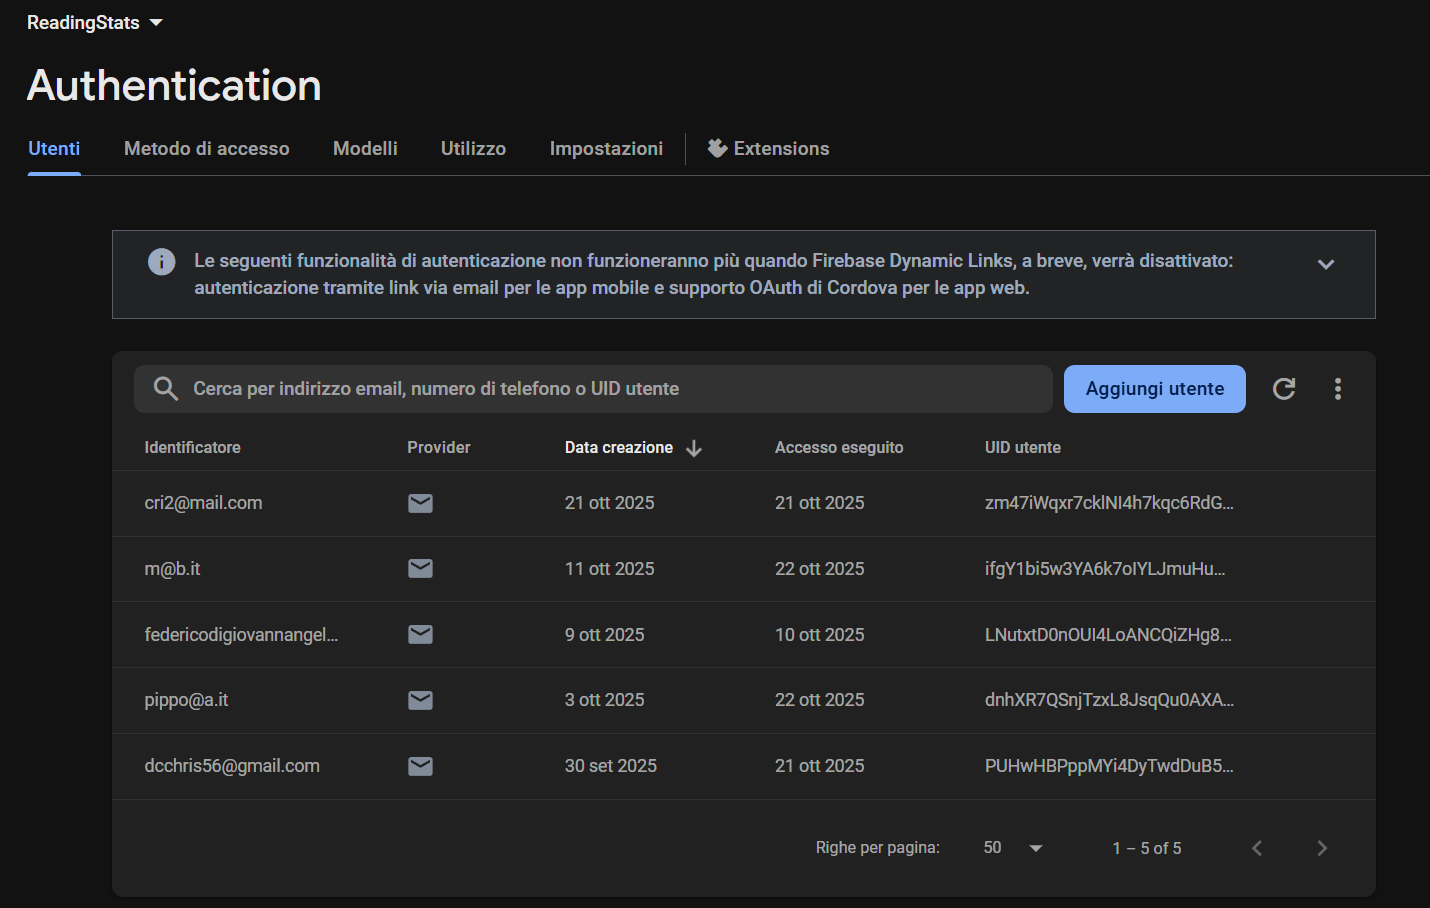
\includegraphics[width=1\linewidth]{authentication.png}
    \caption{Diagramma delle componenti}
    \label{fig:sitemap}
  \end{figure}
  \item \textit{Firestore Database:} permette la memorizzazione tramite documenti e collezioni descritti in precedenza dei dati dell'utente, delle richieste di amicizia inviate tra utenti e dei libri salvati con ognuno la relativa sessione. 
  Sono state implementate delle regole specifiche per permettere un corretto e coerente accesso ai dati e la loro relativa modifica. Di seguito i documenti e le collezioni generate:
  
  \textit{INSERIRE SCREEN PER OGNI SEZIONE}

  \begin{itemize}
    \item \textbf{Salvataggio utenti:} Utenti registrati e salvati nel servizio tramite il form di registrazione, memorizzando nome, cognome, username e mail;
    \item \textbf{Salvataggio usernames:} Username salvati al momento della registrazione per permettere un controllo di univocità;
    \item \textbf{Salvataggio di amici tramite richieste:} Lista di utenti che si aggiorna per ogni singolo utente quando accetta una richiesta di amicizia da un altro utente;
    \item \textbf{Salvataggio di libri dal catalogo:} Raccolta di libri salvati per ogni utente, ognuno con le sue informazioni e lo stato per visualizzarlo in una determinata lista tra quelle fornite;
    \item \textbf{Salvataggio sessione di lettura:} Per ogni libro nello stato "In lettura", viene memorizzata una sessione di lettura contenente il tempo memorizzato in secondi e convertito a schermo in ore:minuti:secondi;
    \item \textbf{Regole di accesso ai documenti definiti:} Le seguenti regole scritte nell'omonima sotto-sezione permettono la definizione di un accesso; 
  \end{itemize} 
\end{itemize}



\subsection{API utilizzate - Google Books}
Le API di Google Books sono state utilizzata per ottenere le informazioni principali dei libri, in modo da permettere
all'utente la loro visualizzazione e il conseguente salvataggio. L'API viene fornita tramite un link 
per le ricerche e una chiave generata da Google Cloud per permetterne l'abilitazione e la limitazione del tipo di dispositivo che la utilizzerà.

\textit{Link:  https://www.googleapis.com/books/v1/volumes?q=search-terms}.

\textit{"q"} è il parametro da inserire per effettuare la ricerca tramite titolo o autore. Sono presenti altri parametri, i cui principali per l'applicazione sono stati:
\begin{itemize}
  \item \textit{maxResults}, per mostrare la quantità di libri da visualizzare, utilizzato in particolare nel catalogo e nella ricerca.
  \item \textit{orderBy}, il quale può essere relevance o newest per mostrare libri di maggiore rilievo tramite parametriche di Google o nuove uscite.
  \item \textit{langRestrict}, ossia la restrizione dei libri da visualizzare e ricercare con la una lingua specifica.
\end{itemize}


\subsection{Sviluppo}
Come anticipato in precedenza, l'applicazione è interamente sviluppata in \textbf{Jetpack Compose}, un toolkit dichiarativo di Android che permette, al variare del proprio stato, di ridisegnare le parti necessarie al cambiamento di tale stato.

Permette un approccio dichiarativo tramite la definizione di funzioni con notazione \textit{@Composable}, le quali permettono di definire parti di interfaccia utente esclusivamente con codice Kotlin. 
In queste funzioni si controlla lo stato per permettere l'aggiornamento di determinate parti coinvolte.

Sono disponibili una serie di layout predefiniti (Column, Row, Box) per strutturare al meglio una componente dell'interfaccia e le funzioni accettano un parametro Modifier che permette di modificarne l'aspetto estetico.

Per la costruzione di un'interfaccia tradizionale è stato utilizzata la funzione \textit{Scaffold} con parametri per definire componenti predefinite come TopAppBar, BottomAppBar, FloatingActionButton e altri ancora.

Si possono distinguere due tipi di funzioni Composable:
\begin{itemize}
  \item \textbf{Stateful}, fa utilizzo della keyword \textit{remember} che permette di memorizzare dati tra diverse recomposition
  \item \textbf{Steless}, ossia un Composable orivo di stato
\end{itemize}

Le liste scorrevoli che visualizzano molti elementi vengono gestite da componenti \textit{Lazy}, che forniscono un blocco per descrivere i singoli \textit{item} da visualizzare.  
Ne esistono diverse versioni:
\begin{itemize}
  \item \textbf{LazyRow} per lo scorrimento orizzontale,
  \item \textbf{LazyColumn} per lo scorrimento verticale,
  \item \textbf{LazyVerticalGrid e LazyHorizontalGrid} per lo scorrimento di una griglia rispettivamente verticale e orizzontale
\end{itemize}

La navigazione viene principalmente gestita tramite un file dedicato, denominato \textbf{AppNavHost.kt},
nel quale viene creato un \textit{NavController} e un \textit{NavHost},
il quale fa uso della funzione \textit{composable} che permette di definire le rotte di destinazione
all'interno dell'applicazione. Tali rotte vengono definite in formato di stringa in un altro file denominato \textbf{Routes.kt} 

Le funzioni con notazione \textit{@Composable} possono essere richiamate da un Activity o Fragment, da altre funzioni \textit{@Composable}, 
all'interno di una destinazione definita in Navigation-Compose e in liste Lazy.

\subsubsection{Struttura package}
Il progetto, strutturato con architettura MVVM, è stato suddiviso in macro-package al cui interno sono presenti file o altri package caratteristici.

La struttura delle macro-cartelle risulta la seguente:

\begin{itemize}
  \item \textbf{core:} contiene i package con i file di parti di interfaccia
  \textit{@Composable} riutilizzabili nel codice e i file utilizzati per la personalizzazione globale dell'app.
  \item \textbf{di:} moduli di \textit{Dependency Injection} (Hilt) che descrivono come creare e fornire le dipendenze dell’app. 
  Le classi ricevono gli oggetti necessari tramite iniezione, senza istanziarli al proprio interno. 
  Contiene i file usati a livello globale per integrare le Google Books API e configurare lo stack di rete.
  \item \textbf{features:} è presente il codice principale dell'applicazione scritto in diversi file distinti e gestito in package annidati per la loro funzionalità nell'applicazione.
  \item \textbf{navigation:} contiene i file di gestione della navigazione e di creazione delle route
\end{itemize}

\subsubsection{File di configurazione}

\subsection{Spiegazione codice in dettaglio}

\subsubsection{core: Componenti Compose riutilizzabili}

\subsubsection{di: Dependency Injection}

\subsubsection{Model dell'applicazione}

\subsubsection{Funzioni composable per l'interfaccia}

\subsubsection{File di definizione del ViewModel}

\subsubsection{Repository}

\subsubsection{UseCases}

\subsection{Unit Testing}

\section{Progettazione e sviluppo in Flutter}

\section{UI - Interfaccia applicazione}

\section{Discussioni di problematiche riscontrate}

\section{Conclusioni}

\end{document}
